%! TEX program = pdflatex

\documentclass[oneside,solution]{tmpl}

\usepackage[utf8]{inputenc}
\usepackage[english,ukrainian]{babel}
\usepackage{float}

\title{Залікова робота}
\author{Захаров Дмитро}
\studentID{МП-31}
\instructor{Ігнатович С.Ю.}
\date{\today}
\duedate{15:00 27 травня, 2024}
\assignno{}
\semester{Весняний семестр 2024}
\mainproblem{Залікова Робота}

\begin{document}

\maketitle

% \startsolution[print]

\problem{Перколяції.}

\hspace{20px}\textbf{Умова.} Процес перколяції: де виникає, як його можна моделювати, залежність від яких параметрів можна досліджувати.

\textbf{Відповідь.} Перед тим, як сформулювати поняття перколяції, давайте трошки опишемо об'єкт, з котрим ми будемо працювати. Зафіксуємо деяку дошку розміру $n \times n$, в кожну клітинку ми будемо ставити одне з двох значень:
\begin{itemize}
    \item 1 -- якщо на цій клітинці знаходиться перешкода.
    \item 0 -- якщо ця клітинка вільна.
\end{itemize}

Далі виникає питання, а за яким правилом ми будемо генерувати такий ``лабіринт''? Розглянемо дуже простий варіант. Нехай $X_{i,j}$ -- значення в клітинці $(i,j)$. Тоді нехай $X_{i,j} \sim \text{Bernouli}(\theta)$, тобто з ймовірністю $0 \leq \theta \leq 1$ будемо мати перешкоду в цій клітинці, а з ймовірністю $1-\theta$ будемо мати вільну клітинку. Отже, з формою лабіринту ми визначилися.

А тепер поставимо таке питання: нехай ми поставили персонажа у якусь з клітинок найвищого рядка $X_{i,1},\; i = 1,\dots,n$. Яка ймовірність, що персонаж зможе пройти лабіринт, якщо вихід знаходиться під найнижчим рядком $X_{i,n}, \;i = 1,\dots,n$.

Зазначимо, що це дещо іграшкова аналогія і такий процес можна використовувати у дійсно прикладних задачах. Наприклад, якщо вважати за $1$ -- клітинки з діелектриком, а за $0$ -- провідник, то наявність шляху зверху вниз може означати, що струм зможе пройти по цій ділянці. Або, замість персонажа можна пускати воду, тоді питання буде полягати в тому, чи пройде вода через задану ділянку. 

Далі використаємо аналогію з провідником і на ній проілюструємо, чому така проблема є важливою. Нехай в нас є електричне коло, що зображено на Рисунку \ref{fig:problem_1_illustration}.

\begin{figure}[H]
    \centering
    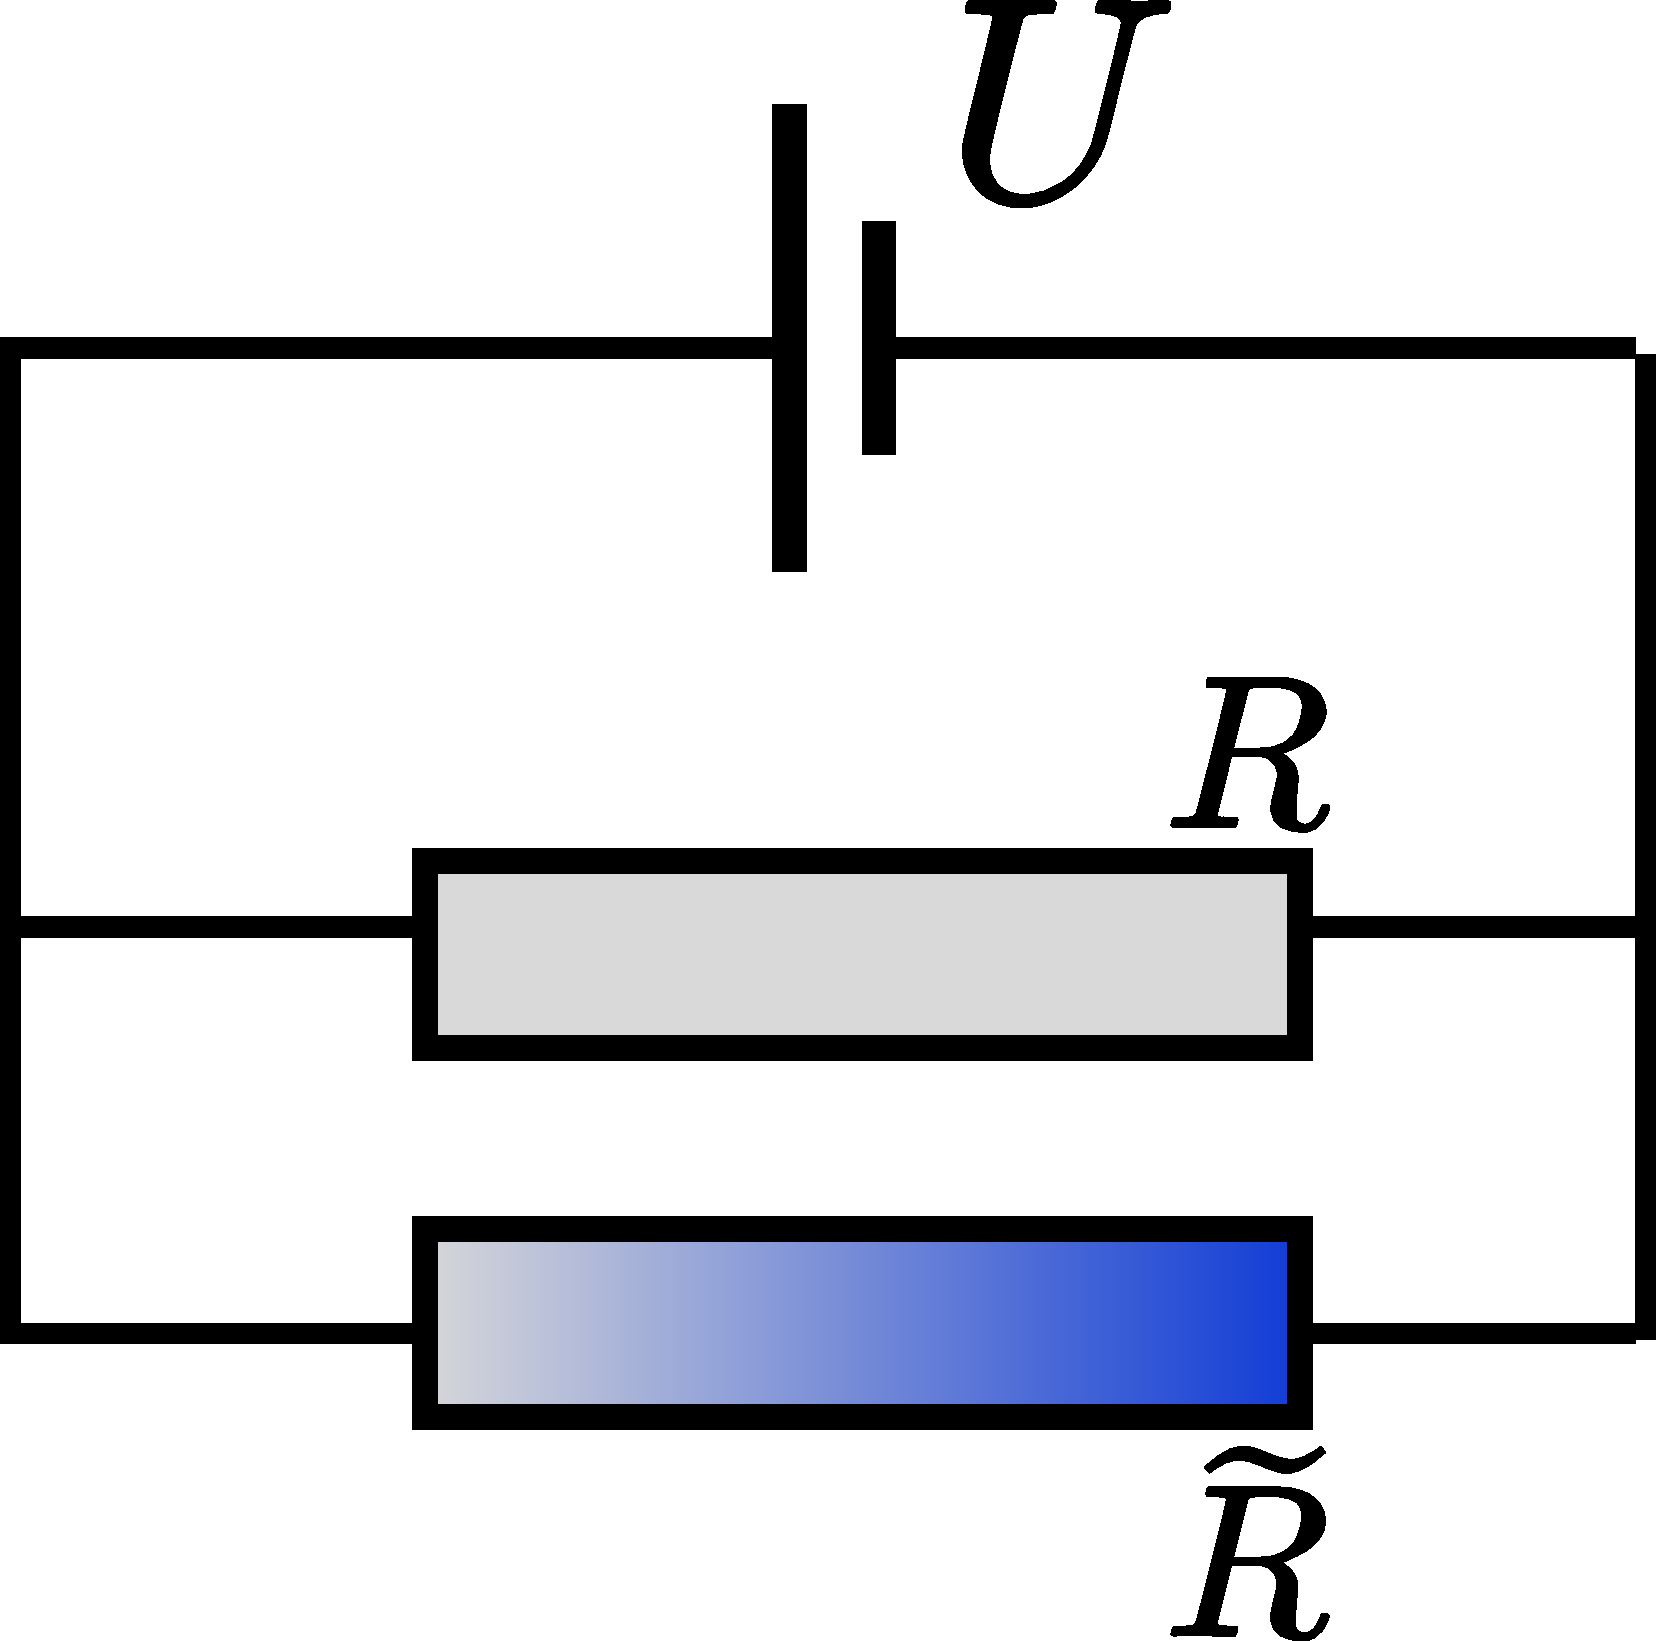
\includegraphics[width=0.3\textwidth]{images/exam/circuit.pdf}
    \caption{Ілюстрація явища перколяції}
    \label{fig:problem_1_illustration}
\end{figure}

Нехай $R$ -- супротив звичайного резистора, а $\widetilde{R}(\theta)$ -- того, який моделюється за допомогою алгоритму з клітинками вище (назвемо його нелінійним). Дуже спрощено, нехай ми почали експеримент, тоді фікується $\widetilde{R} = 0$, якщо знайшовся шлях по нелінійному елементу, а інакше фіксуємо $\widetilde{R} = R_0$. 

Тепер під'єднаємо амперметр до кола послідовно і будемо міряти його показання. Якщо ми будемо плавно змінювати $R$, то і значення амперметру буде плавно змінюватись\footnote{Якщо точніше, то наближено $I = U(R+\widetilde{R}(\theta))/R\widetilde{R}(\theta)$.}. Тобто, графік $I(R)$ буде певною неперервною величиною -- це ми добре знаємо зі шкільної фізики. А тепер цікаве наступне питання: а яка буде залежність середнього значення току від $\theta$\footnote{Оскільки сама $I$ є випадковою величиною, то тут ми скоріше говоримо про математичне сподівання $\mathbb{E}[I]$, але не будемо сильно вдаватись у деталі.}?

Зрозуміло, що для $\theta$, близьких до 1, скоріше за все супротив нелінійного елемента стане $R_0$ і ток буде дорівнювати $U(R+R_0)/RR_0$. Якщо ж, навпаки, $\theta$ близьке до $0$, то ток буде протікати по всьому колу без супротиву і амперметр скоріше за все поламається, оскільки $I \to \infty$ :) 

А ось цікаво -- на якому саме етапі відбувається цей перехід між скінченним значенням і ``вибухом''? Цей фазовий перехід, в якому відбувається дуже різка зміна середовища (в нашому випадку, наприклад, електричного кола) і називається \textbf{перколяцією} (походить від геологічного терміну -- протікання/фільтрування рідини). 

Конкретно наша задача з решіткою називається \textbf{задача вузлів}, а ланцюжок знизу вверх називають \textbf{перколяційним кластером}. Також, хоча ми і розглядали квадратну решітку $n \times n$, на практиці часто використовують і більш-вимірні моделі, наприклад паралелепіпед $a \times b \times c$. Проте, виявляється, що навіть для двовимірної простої моделі задача аналітично нерозв'язана.

Але експериментально досліджувати достатньо легко: зафіксуємо певне $\theta \in [0,1]$ і проводимо багато експериментів, в кожному з яких генеруємо поле і далі перевіряємо ``в лоб'', чи виникла перколяція. Досліджувати можна, наприклад, частку виникнення перколяцій від параметру $\theta$ або середня максимальна глибина ``занурення''. Цікаво, що при цьому графіки виходять дуже ``обривистими'' -- тобто при якомусь $\theta$ частка різко з $1$ переходить до $0$. Також можна, наприклад, змінювати розмір поля (тобто параметр $n$), робити поле неквадратним, або навіть об'ємним. Нарешті, ніхто не заважає змінити розподіл клітинок $X_{ij}$ зі стандартного Бернулівського, як ми це описували, на щось більш цікаве :)

\problem{Фазові портрети.}
\hspace{20px}\textbf{Умова.} Фазові портрети двовимірних лінійних систем. Поясніть, як у випадку фокусу або центру
дізнатися напрям обертання. У випадку сідла: як знайти сепаратриси?

\textbf{Відповідь.} Нехай ми маємо деякий процес. Цей процес описується деяким вектором величин $\mathbf{x} = (x_1,\dots,x_n)$ (наприклад, $x_1$ -- це координата, а $x_2$ -- це швидкість) і ми знаємо закон, котрий описує як динамічно змінюється ця система:
\begin{equation}
    \dot{\mathbf{x}} = f(\mathbf{x}, t),
\end{equation}

де $f: \mathbb{R}^n \times \mathbb{R}_{\geq 0} \to \mathbb{R}^n$ -- деяка (нехай неперервна) функція. Далі сконцентруємось на дуже простому випадку функції $f$. Нехай $f(\mathbf{x},t) = \boldsymbol{A}\mathbf{x}$, тобто наше рівняння має вигляд
\begin{equation}\label{eq:linear_system}
    \dot{\mathbf{x}} = \boldsymbol{A}\mathbf{x}
\end{equation}

\textit{Зауваження:} було б можливо більш чесно розглядати систему $\dot{\mathbf{x}} = \boldsymbol{A}\mathbf{x} + \mathbf{b}$, проте її легко можна звести до вигляду \ref{eq:linear_system} лінійною заміною змінних.

Таке рівняння називають \textbf{лінійною системою}. Дослідження таких систем є дуже корисним як мінімум з двох причин:
\begin{itemize}
    \item Дуже багато систем в прикладних задачах описується саме лінійним законом (або можуть бути спрощені до таких), котрий дуже зручно і легко досліджувати.
    \item Навіть у випадку нелінійних функцій $f$, їх можна лінеаризувати і досліджувати деякі околи, що нас цікавлять.
\end{itemize}

Проте, спростимо задачу ще далі і будемо вважати $n=2$, тобто маємо двовимірний випадок. Ключове питання: як будуть виглядати фазові портрети таких систем?

Почнемо досліджувати. Звичайно, якщо вважати $\boldsymbol{A} = \begin{bmatrix}
    a_{1,1} & a_{1,2} \\ a_{2,1} & a_{2,2}
\end{bmatrix}$ і аналізувати Рівняння \ref{eq:linear_system} в залежності від усіх $a_{i,j}$, то можна злетіти з катушок, бо параметрів ну надто багато. Тому тут нам дещо допоможе курс лінійної алгебри, а саме тема діагоналізації матриць.

Нехай маємо власні числа $\lambda_1,\lambda_2$ матриці $\boldsymbol{A}$, причому $\lambda_1 \neq \lambda_2 > 0$. Нехай відповідні власні вектори $\mathbf{v}_1$ та $\mathbf{v}_2$. Введемо допоміжну матрицю, що складена з власних векторів $\boldsymbol{U} = (\mathbf{v}_1 \parallel \mathbf{v}_2)$ і зробимо ось таку зручну заміну змінних: $\mathbf{z} = \boldsymbol{U}^{-1}\mathbf{x} \implies \mathbf{x} = \boldsymbol{U}\mathbf{z}$. Тожі, наша система \ref{eq:linear_system} набуде вигляду:
\begin{equation}
    \boldsymbol{U}\dot{\mathbf{z}} = \boldsymbol{A}\boldsymbol{U}\mathbf{z} \implies \dot{\mathbf{z}} = (\boldsymbol{U}^{-1}\boldsymbol{AU})\mathbf{z}
\end{equation}

А далі помічаємо дуже зручну для нас річ. Відомо, що при нашому виборі матриці $\boldsymbol{U}$ вираз $\boldsymbol{U}^{-1}\boldsymbol{AU}$ дорівнює діагональній матриці $\text{diag}\{\lambda_1, \lambda_2 \}$. І тому система набула вигляду:
\begin{equation}\label{eq:linear_system_simplified}
    \begin{cases}
        \dot{z}_1 = \lambda_1 z_1 \\
        \dot{z}_2 = \lambda_2 z_2
    \end{cases}
\end{equation}

Помітимо, що характеристичні властивості, що ми виведемо для Рівняння \ref{eq:linear_system_simplified} будуть аналогічні для Рівняння \ref{eq:linear_system}, оскільки ми зробили звичайне лінійне перетворення. Це рівняння дуже легко розв'язати: отримуємо траєкторію:
\begin{equation}\label{eq:trajectory}
    z_1(t) = c_1e^{\lambda_1 t}, \; z_2(t) = c_2e^{\lambda_2 t}
\end{equation}

Власне, ми вже отримали розв'язок для випадку $\lambda_1 \neq \lambda_2 > 0$. Проте, отримана траєкторія може набувати трьох різних ``характерних'' форм. Щоб це побачити, випишемо рівняння у вигляді $z_2=g(z_1)$. З першого рівняння $t = \frac{1}{c_1}\log \frac{z_1}{\lambda_1}$, а тому підставляючи у друге отримаємо:
\begin{equation}
    z_2 = c_2 \left(\frac{z_1}{c_1}\right)^{\lambda_2 / \lambda_1} = r \cdot |z_1|^{\lambda_2/\lambda_1},
\end{equation}

де $r$ -- це якась константа. Бачимо, що взаємозв'язок між $z_1$ та $z_2$ степеневий, і тому найбільш цікавий момент -- це степінь $\lambda_2/\lambda_1$. Отже, природньо розглянути наступні випадки:
\begin{itemize}
    \item Якщо $\lambda_1, \lambda_2 > 0$, тоді показник додатний і фазовий портрет виглядає як ``напівпараболи'' і напівпрямі, що проходять через $(0,0)$. Також, з Рівняння \ref{eq:trajectory} видно, що $z_1,z_2 \to \infty$, тому траєкторія буде виходити кудись на нескінченність. Це означає, що точка $(0,0)$ нестійка і тому такий випадок називають \textbf{нестійким вузлом}.
    \item Якщо $\lambda_1 < 0 < \lambda_2$, то показник від'ємний і це буде відповідати ``півгіперболам''. Такий випадок називають \textbf{сідлом}. Напівпрямі тут мають доволі важливу роль, тому їх називають \textbf{сепаратрисами}. Про них окремо поговоримо.
    \item Якщо $\lambda_1,\lambda_2 < 0$, то показник знову додатний і ми маємо ``напівпараболи''. Це також вузол, але вже стійкий: видно, що $z_1,z_2 \to 0$ через те, що показники в експоненті від'ємні.
\end{itemize}

Отже, випадок дійсних $\lambda_1,\lambda_2$ розглянули. Тепер нехай $\lambda_1 = u+iv \in \mathbb{C}$, тоді $\lambda_2 = \overline{\lambda}_1 = u-iv$. Тоді з курсу лінійної алгебри відомо, що $\boldsymbol{U}^{-1}\boldsymbol{A}\boldsymbol{U} = \begin{bmatrix}
    u & v \\ -v & u
\end{bmatrix}$, тому наша система набуде вигляду
\begin{equation}
    \begin{cases}
        \dot{z}_1 = uz_1 + vz_2 \\
        \dot{z}_2 = -vz_1 + uz_2
    \end{cases}
\end{equation}

Найпростіше розглянути $u=0$, тобто наші комплексні числа чисто комплексні ($\lambda_1,\lambda_2 \in \mathbb{C} \setminus \mathbb{R}$). Тоді система має вигляд
\begin{equation}
    \begin{cases}
        \dot{z}_1 = vz_2 \\
        \dot{z}_2 = -vz_1
    \end{cases}
\end{equation}

Це рівняння зводиться до $\ddot{z}_1 + v^2z_1 = 0$, що відповідає гармонічним коливанням з частотою $v$. Тому, $z_1 = z_m \cos (vt + \phi)$, де $z_m$ -- амплітуда, а $\phi$ -- фазовий зсув. Тоді $z_2(t) = -A \sin (vt + \phi)$. Дуже легко тепер бачити, що $(z_1(t), z_2(t))$ описують кола радіуса $R$, тобто наші фазові траєкторії -- це кола різних радіусів навколо $(0,0)$. Цей випадок називають \textbf{центром}.

При $u \neq 0$ все складно. Тут легше перейти до полярних координат: нехай $z_1=\rho \cos \theta, z_2=\rho \sin \theta$, тоді наше рівняння зведеться до (викладки пропустимо, оскільки вони доволі громіздкі):
\begin{equation}
    \begin{cases}
        \dot{\rho} = u\rho \\
        \dot{\varphi} = -v
    \end{cases}
\end{equation}

Отже, по суті в нас два незалежних рівняння. Друге описує обертання з постійною кутової швидкістю навколо $(0,0)$, а знак $v$ показує орієнтацію обертання. Дійсно, якщо $v<0$, то кутова швидкість $\dot{\varphi}$ постійна і додатна, а отже обертання відбувається проти годинникової стрілки. Відповідно, якщо $v>0$, то кутова швидкість від'ємна і тому обертання йде за годинниковою стрілкою.

В свою чергу знак $u$ показує, куди саме прямує точка -- до $(0,0)$ чи від $(0,0)$, оскільки $\rho(t) = \rho_m e^{ut}$. Якщо $u < 0$ (тобто $\text{Re}(\lambda_1) = \text{Re}(\lambda_2) < 0$), то траєкторія стабільна -- точка закручується ``у центр'', а інакше нестабільна. Такі два випадки називають \textbf{стійким фокусом} та \textbf{нестійким фокусом}, відповідно. 

\textbf{Код на Python.} Давайте проілюструємо всю класифікацію на мові \textit{Python}. Для цього зробимо ілюстрацію дещо цікавішою: ми звикли, що зазвичай ілюстрації проводять для діагональних матриць, тому сепаратриси та характерні прямі вертикальні/горизонтальні. Тому, зробимо матрицю меньш тривіальною. Зафіксуємо матрицю повороту:
\begin{equation}
    \boldsymbol{R} = \begin{bmatrix}
        \cos \frac{\pi}{6} & -\sin \frac{\pi}{6} \\
        \sin \frac{\pi}{6} & \cos \frac{\pi}{6}
    \end{bmatrix}
\end{equation}

і в якості матриці для лінійної системи візьмемо $\boldsymbol{R}^{-1}\cdot\text{diag}(\lambda_1,\lambda_2)\cdot\boldsymbol{R}$ для обраних $\lambda_1,\lambda_2$. Ми так можемо робити, бо операція $\boldsymbol{R}^{-1}(\star) \boldsymbol{R}$ не змінює спектр матриці, а отже характеристика портрету буде зберігатись. 

Отже, програма для цього:
\begin{lstlisting}[language=Python]
import numpy as np
import matplotlib.pyplot as plt

from typing import Tuple, List

def draw_streamplot(ax: plt.axes, 
                    title: str,
                    f: callable, 
                    stationary_points: List[Tuple[float, float]] = []) -> None:
    """
    Draws a streamplot on the provided axes based on the vector field provided.
    
    Args:
    - `ax` - the axes object to draw the streamplot on
    - `title` - title of the plot
    - `f` - the vector field function
    - `stationary_points` - a list of stationary points to be marked on the plot. Empty by default.
    
    Output:
    `None`, modifies the provided ax
    """
    
    # Some fancy customizations
    ax.set_aspect('equal')
    ax.grid()
    ax.set_title(title)
    
    # Drawing the streamplot
    x = np.linspace(-3.0, 3.0, 50) # Choosing the range of x 
    y = np.linspace(-3.0, 3.0, 50) # Choosing the range of y
    xx, yy = np.meshgrid(x,y) # Creating a meshgrid
    f1, f2 = f(xx,yy) # Calculating the vector field
    ax.streamplot(xx, yy, f1, f2, density=1.8, color='b') # Drawing a phase portrait
    
    # Drawing the stationary points
    for point in stationary_points:
        ax.scatter(point[0], point[1], color='red', marker='x', alpha=1.0, s=100, linewidths=3.0, zorder=10)
    

if __name__ == '__main__':
    # Define a matrix that will be used to make the matrix of the
    # linear system less obvious by taking A^{-1}diag(lambda_1, lambda_2)A
    # Here, this is just a rotational matrix by pi/6
    A = np.matrix([[np.cos(np.pi/6), -np.sin(np.pi/6)], [np.sin(np.pi/6), np.cos(np.pi/6)]]) 
    A_inv = np.linalg.inv(A)
    
    # Defining the vector field functions for each of the cases
    def stable_node(x: np.ndarray, y: np.ndarray) -> callable:
        # Here, both eigenvalues are negative
        lambda_1 = -1
        lambda_2 = -1.5
        matrix = A_inv @ np.matrix([[lambda_1, 0], [0, lambda_2]]) @ A
        return matrix[0, 0] * x + matrix[0, 1] * y, matrix[1, 0] * x + matrix[1, 1] * y
    
    def saddle(x: np.ndarray, y: np.ndarray) -> callable:
        # Here, one eigenvalue is negative and one is positive
        lambda_1 = -1.0
        lambda_2 = 4.0
        matrix = A_inv @ np.matrix([[lambda_1, 0], [0, lambda_2]]) @ A
        return matrix[0, 0] * x + matrix[0, 1] * y, matrix[1, 0] * x + matrix[1, 1] * y
    
    def center(x: np.ndarray, y: np.ndarray) -> callable:
        # Here, both eigenvalues are pure complex
        v = 4.0
        matrix = A_inv @ np.matrix([[0, v], [-v, 0]]) @ A
        return matrix[0, 0] * x + matrix[0, 1] * y, matrix[1, 0] * x + matrix[1, 1] * y
    
    def unstable_focus(x: np.ndarray, y: np.ndarray) -> callable:
        # Here, both eigenvalues are complex with positive real part
        u = 3.0
        v = 6.0
        matrix = A_inv @ np.matrix([[u, v], [-v, u]]) @ A
        return matrix[0, 0] * x + matrix[0, 1] * y, matrix[1, 0] * x + matrix[1, 1] * y
    
    # Plotting all phase portraits
    fig, axs = plt.subplots(2, 2)
    fig.set_figheight(10)
    fig.set_figwidth(10)
    
    # Modifying subplots
    draw_streamplot(axs[0, 0], 'Stable node\n(λ1=-1.0, λ2=-1.5)', stable_node, stationary_points=[(0.0, 0.0)])
    draw_streamplot(axs[0, 1], 'Saddle point\n(λ1=-1.0, λ2=4.0)', saddle, stationary_points=[(0.0, 0.0)])
    draw_streamplot(axs[1, 0], 'Center\n(λ1=4.0i, λ2=-4.0i)', center, stationary_points=[(0.0, 0.0)])
    draw_streamplot(axs[1, 1], 'Focus\n(λ1=3.0+6.0i, λ2=3.0-6.0i)', unstable_focus, stationary_points=[(0.0, 0.0)])
    
    # Saving the figure
    fig.savefig(f'exam_problem_2.pdf')
\end{lstlisting}

А тепер розглянемо отриману ілюстрацію -- дивись Рисунок \ref{fig:problem_2_illustration}.

\begin{figure}[H]
    \centering
    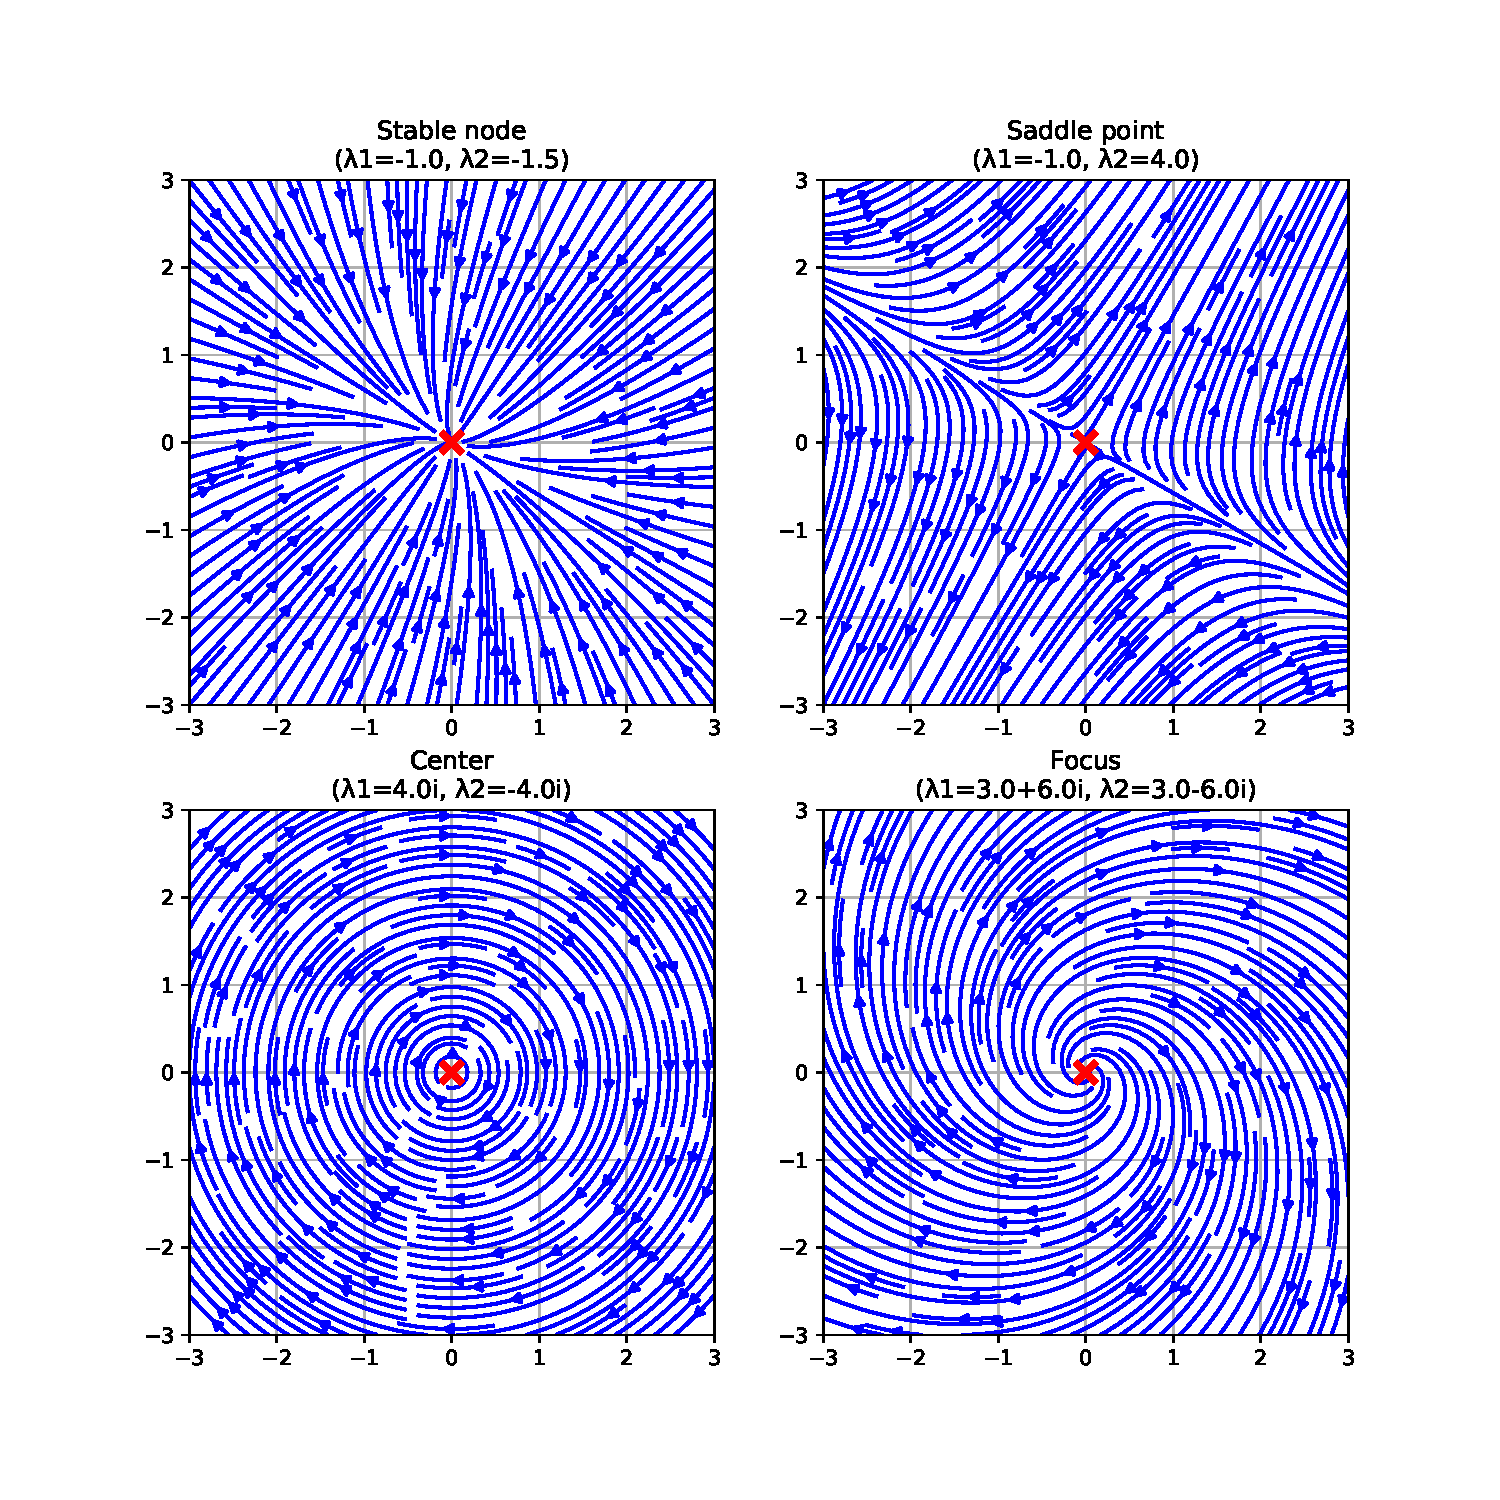
\includegraphics[width=0.8\textwidth]{images/exam/exam_problem_2.pdf}
    \caption{Ілюстрація чотирьох основних фазових портретів (без врахування стабільності/нестабільності)}
    \label{fig:problem_2_illustration}
\end{figure}

Зауважимо, що тут можна ще додати нестійкий вузол та стійкий фокус, але вони, окрім напрямку стрілок, нічим не відрізняються від наведених.

\textbf{Визначення напрямку сепаратрис.} Нагадаємо, що для $\lambda_1 < 0 < \lambda_2$ після заміни $\mathbf{z} = \boldsymbol{U}^{-1}\mathbf{x}$ ми отримали рівняння 
\begin{equation}
    \begin{cases}
        \dot{z}_1 = \lambda_1 z_1 \\
        \dot{z}_2 = \lambda_2 z_2
    \end{cases}
\end{equation}

Для нього маємо дві сепаратриси: $z_1=0$ та $z_2=0$. Дійсно, якщо наприклад $z_1(0)=0$, то $z_2 = c_2e^{\lambda_2 t}$ -- маємо рух вздовж $z_1=0$ від $(0,0)$. Аналогічно для $z_2(0)=0$ будемо мати рух вздовж $z_2=0$ до $(0,0)$, оскільки $\lambda_1<0$.

Як отримати рівняння сепаратриси для системи координат $\mathbf{x}$? Дуже просто: нехай маємо сепаратрису $z_1=0$. Тоді вектор нормалі цієї сепаратриси $\boldsymbol{\nu}_z = (0,1)$. У системі $\mathbf{x}$ цей вектор набуде вигляду $\boldsymbol{\nu}_x = \boldsymbol{U}\boldsymbol{\nu}_z$. Отже тепер сепаратриса це просто пряма $\langle \boldsymbol{\nu}_x, \mathbf{x} \rangle = 0$. Аналогічно для $z_2=0$, але тут нормаль $\boldsymbol{\nu}_z = (1, 0)$. Якщо побудувати відповідні прямі для нашої обраної матриці повороту, то отримаємо Рисунок \ref{fig:problem_2_addition}.

\begin{figure}[H]
    \centering
    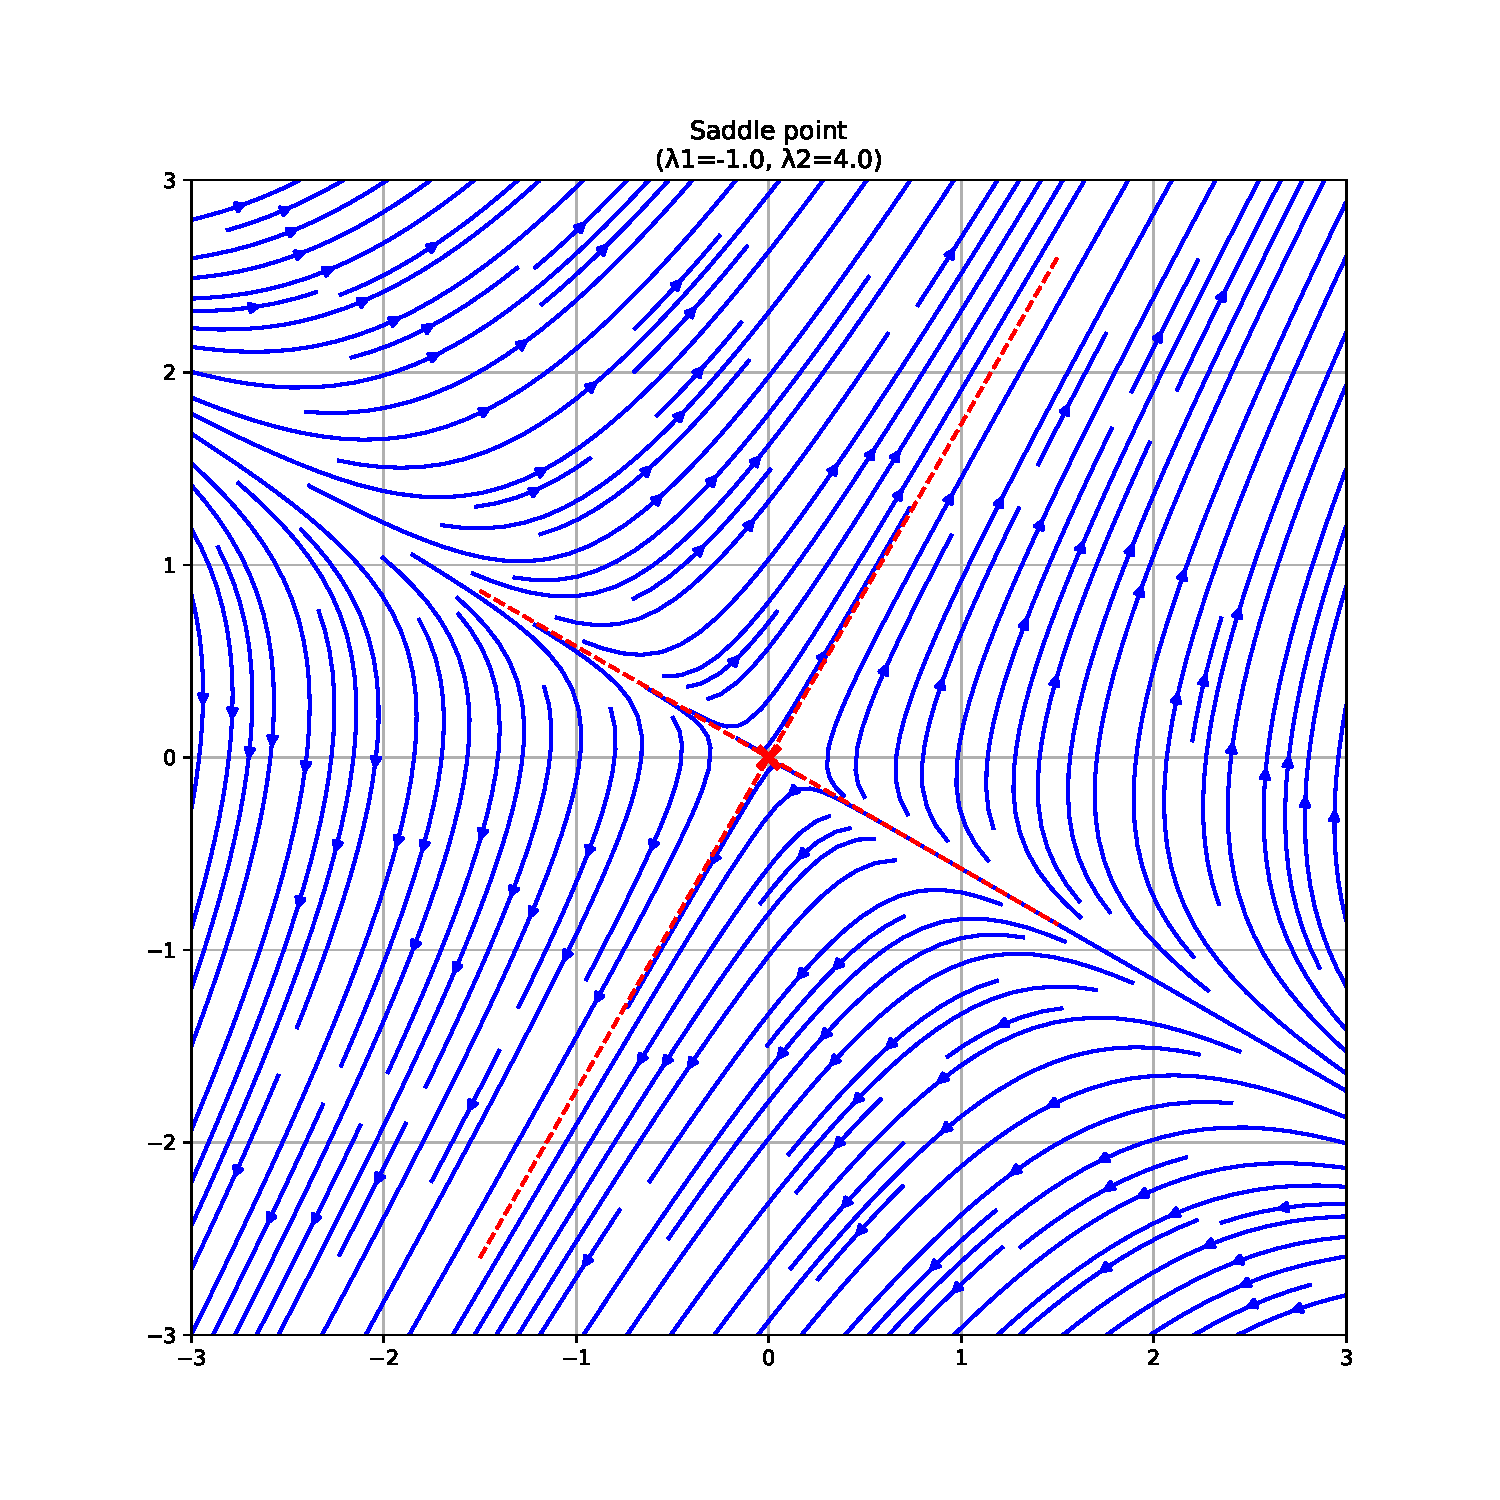
\includegraphics[width=0.7\textwidth]{images/exam/exam_problem_2_2.pdf}
    \caption{Сепаратриси для матриці повороту на кут $\pi/6$.}
    \label{fig:problem_2_addition}
\end{figure}

\end{document}
